Sorting high volumes of products is commonplace in key areas and industries. This text proposes a conveyor system for sorting items based on their sizes. The proposal provides a set of required devices, describes its assembly in a conveyor and continues by presenting a tested prototype simulator that implements the key areas of the proposed system. The text finishes by bringing to light security concerns and explains how they were solved.

The functionality of the system is based on sensors working together to identify, sort and move products into three different lines considering their category A, B or C. This can be done through a conveyor system controlled by a PLC, which uses ladder logic alongside several input and output components to accomplish such a task.

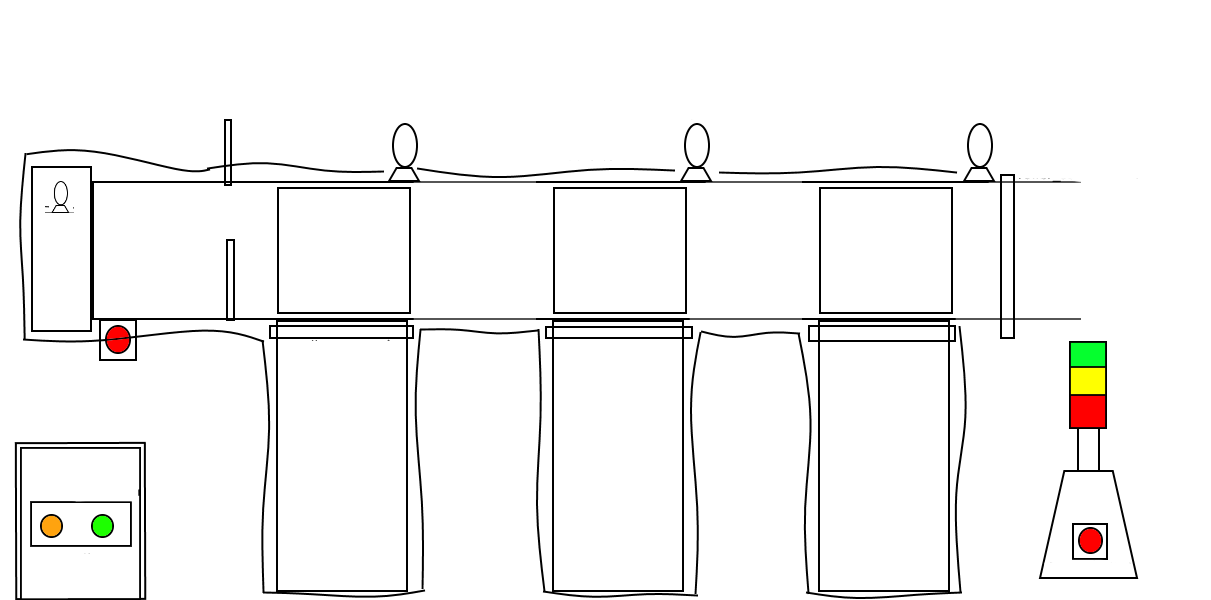
\includegraphics[scale=0.5]{../external/system_graphics_basic.png}